\chapter{Resultados}\label{cap:results}

\section{Regressão Linear Múltipla e Modelo de Regressão em Árvore}

O primeiro experimento definido para este trabalho foi o estabelecimento de uma linha de base para que fosse possível comparar o desempenho de outras abordagens com a base de dados selecionada. Em todas as Figuras, os valores em negritos significam os melhores valores avaliados naquela comparação.

%Initially, the previous analysis consists of choosing between MLRM and RTM as baseline for the next analysis. It could be performed after discussing the information provided in Table \ref{tab:lm_descriptive} and in Figure \ref{fig:mlrm_result}. 
Inicialmente, esse experimento consistiu na seleção entre MRLM e MRA como linha de base. Isso pode ser realizado após discutir a informação apresentada na Tabela \ref{tab:lm_descriptive} e na Figura \ref{fig:mlrm_result}.

%Table \ref{tab:lm_descriptive} shows descriptive statistics of normalized MAE's to both algorithms. Average, standard deviation, minimum and maximum value are calculated for MLRM (cv.lm.v1), $RTM_1$ (cv.rpart.v1), $RTM_2$ (cv.rpart.v2) and $RTM_3$ (cv.rpart.v3). $RTM_1$, $RTM_2$ and $RTM_3$ are regression tree models instances automatically generated by R in this analysis. MLRM has minor values for all statistics.
A Tabela \ref{tab:lm_descriptive} mostra a estatística descritiva do REMQ normalizado para ambos os algoritmos. Os valores de média, desvio padrão, mínimo e máximo são calculados para um Modelo de Regressão Linear Múltipla e três Modelos de Regressão em Árvore: MRLM (cv.lm.v1), $MRA_1$ (cv.rpart.v1), $MRA_2$ (cv.rpart.v2) e $MRA_3$ (cv.rpart.v3).

\begin{table}[h]
\caption{Estatísticas descritivas para erros normalizados dos modelos de regressão linear.}\label{tab:lm_descriptive} \centering
\begin{tabular}{|c|c|c|c|c|}
  \hline
   & MRLM & $MRA_1$ & $MRA_2$ & $MRA_3$ \\
  \hline
  Média & \textbf{0,09912} & 0,10238 & 0,10305 & 0,10361  \\
  \hline
  Desvio Padrão & \textbf{0,00391} & 0,00423 & 0,00441 & 0,00426  \\
  \hline
  Mínimo & \textbf{0,08956} & 0,09214 & 0,09321 & 0,09372  \\
  \hline
  Máximo & \textbf{0,10746} & 0,11231 & 0,11267 & 0,11359  \\
  \hline
\end{tabular}
\end{table}

\begin{figure}[h]
  \vspace{-0.2cm}
  \centering
  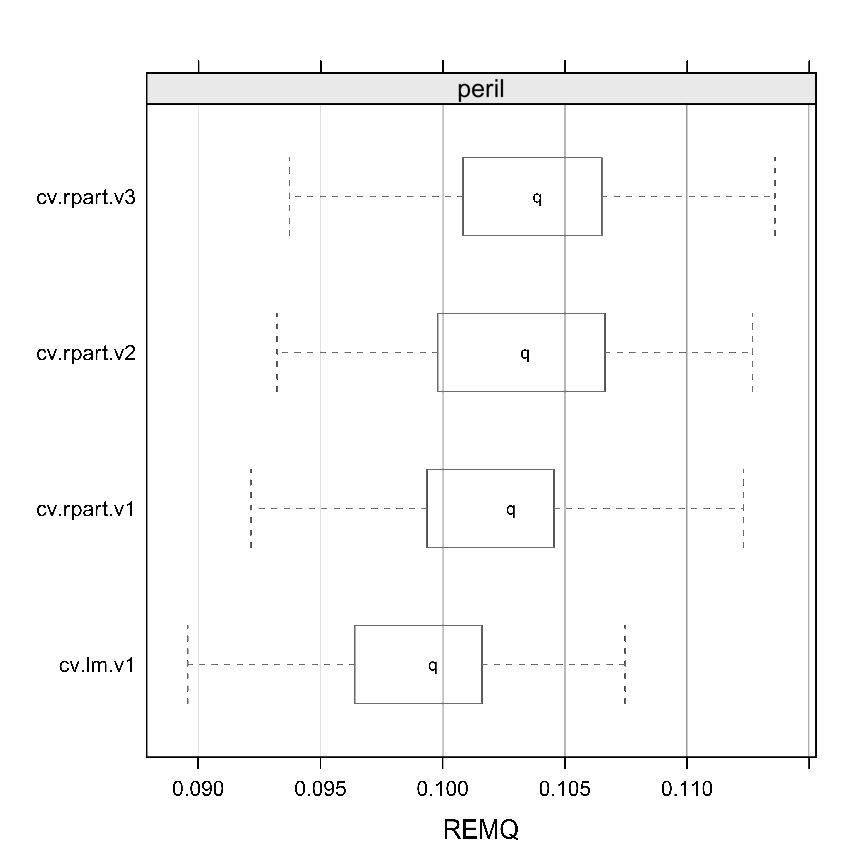
\includegraphics[width=\columnwidth]{image/mrl_ex1.pdf}
  \caption{\textit{Boxplots} para erros normalizados dos modelos de regressão linear, em que MRLM é ``cv.lm.v1", $MRA_1$ é ``cv.rpart.v1", $MRA_2$ é ``cv.rpart.v2" e $MRA_3$ é ``cv.rpart.v3".}
  \label{fig:mlrm_result}
\end{figure}

%In Figure \ref{fig:mlrm_result}, normalized MAE's boxplots after predictions for $RTM_3$, $RTM_2$, $RTM_1$ and MLRM are presented. The minor MAE is obtained on MLRM, this regression model also has minor standard deviation. From those information, we can affirm MLRM is a more efficient and precise model and will be introduced in the experiment as baseline method.
Na Figura \ref{fig:mlrm_result}, os \textit{boxplots} da REMQ normalizada, após as previsões para MRLM, $MRA_1$, $MRA_2$ e $MRA_3$, são apresentados. Os menores valores de média, desvio padrão, mínimo e máximo da REMQ foi obtido para o MRLM, destacados em negrito. A partir dessa informação, pode-se afirmar que o MRLM é um modelo eficiente e preciso. Portanto, é definido como modelo de linha de base.

Os \textit{boxplots} são elementos gráficos bastante utilizados em estudos estatísticos. Eles representam algumas medidas estatísticas como a mediana, o intervalo inter-quartil, os \textit{whiskers} superiores e inferiores e os \textit{outliers}. De modo geral, quanto menor o retângulo, menor o intervalo inter-quartil e o desvio padrão; e quanto menor a mediana, menor a média.

\section{Simulação de Monte Carlo e Análise PERT}

O segundo experimento consiste em analisar o desempenho das técnicas convencionais, Simulação de Monte Carlo e Análise PERT, utilizadas na academia e na indústria, determinadas como boas práticas pelo PMBOK \cite{PMBOK2008}. Como explicado anteriormente, essas abordagens foram configuradas para obterem o melhor desempenho possível.

A Tabela \ref{tab:arte_descriptive} mostra a estatística descritiva da REMQ normalizada para ambos os algoritmos. Os valores de média, desvio padrão, mínimo e máximo, calculados para Simulação de Monte Carlo e para a Análise PERT, mostram que o último apresentou valores bem inferiores de média (0,07466), mínimo (0,04788) e máximo (0,09122). No entanto, o desvio padrão da Simulação de Monte Carlo é inferior (0,01250), provando ser um método mais preciso.

\begin{table}[h]
\caption{Estatísticas descritivas dos erros normalizados para modelos do estado da arte.}\label{tab:arte_descriptive} \centering
\begin{tabular}{|c|c|c|}
  \hline
   & SMC & PERT \\
  \hline
  Média & 0,12640 & \textbf{0,07466}   \\
  \hline
  Desv. Padrão & \textbf{0,01250} & 0,01438   \\
  \hline
  Mínimo & 0,10410 & \textbf{0,04788}   \\
  \hline
  Máximo & 0,14950 & \textbf{0,09122}   \\
  \hline
\end{tabular}
\end{table}

\begin{figure}[h]
  \vspace{-0.2cm}
  \centering
  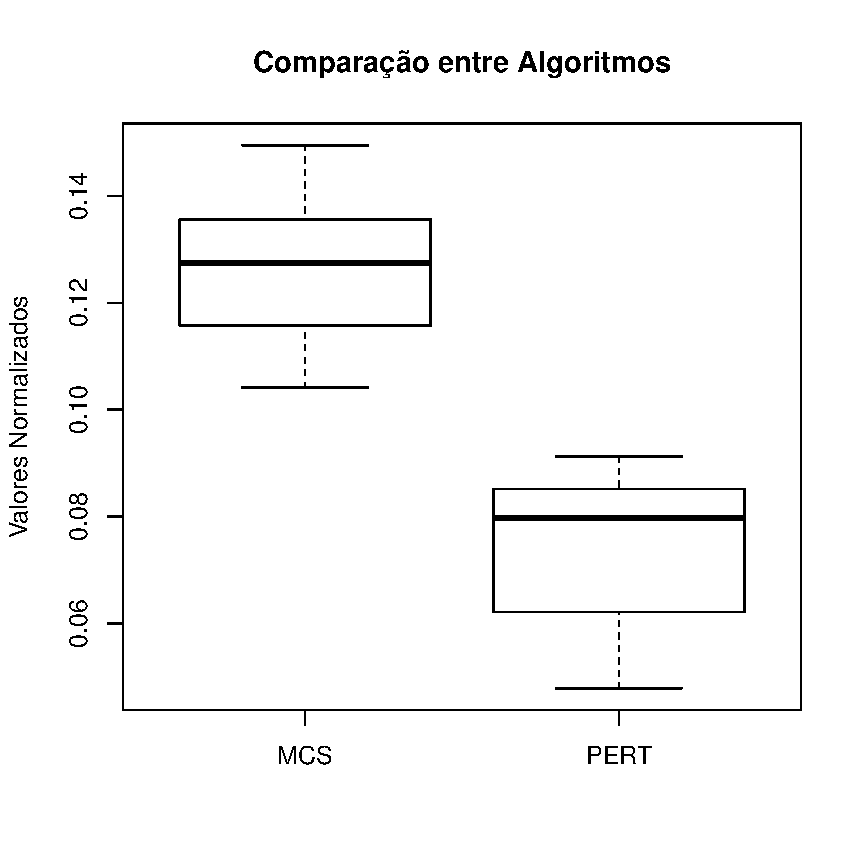
\includegraphics[trim = 1mm 12mm 1mm 1mm,clip,width=0.7\columnwidth]{image/arte_ex2.pdf}
  \caption{\textit{Boxplots} para erros normalizados dos modelos de regressão linear.}
  \label{fig:arte_result}
\end{figure}

Na Figura \ref{fig:arte_result}, os \textit{boxplots} da REMQ normalizada, após as previsões para SMC e PERT, são apresentados. A partir dessa informação, pode-se afirmar que a Análise PERT é um modelo de estado da arte mais eficaz 40\% na média, porém, menos preciso 40\% quanto ao desvio padrão quanto ao REMQ comparado com o SMC.

A Análise PERT mostrou ser uma abordagem bastante interessante quando há poucas informações sobre riscos nas lições aprendidas no gerenciamento de projetos anteriores, por meio de uma base de dados de registro de riscos. Uma análise detalhada utilizando uma base de dados revela que essa técnica apresenta resultados aceitáveis pelos gerentes de projetos.

\section{Perceptron de Múltiplas Camadas e suas variações}

Nesse experimento, algumas MLPs foram avaliadas, sendo a principal diferença entre elas a regra de aprendizagem. Os algoritmos \textit{Backpropagation}, Levenberg-Marquardt, Broyden-Fletcher-Goldfarb-Shanno \textit{Backpropagation}, Gradiente Conjugado Escalonado, \textit{Resilient-propagation}, \textit{One-step Secant backpropagation} e Quasi-Newton foram algumas das regras selecionadas.

Na Tabela \ref{tab:mlps_descriptive}, é exibida a estatística descritiva da REMQ normalizada para as abordagens desenvolvidas para esse experimento. Os valores de média, desvio padrão, mínimo e máximo são calculados para cada uma das MLPs. BP apresenta os resultados para uma MLP com algoritmo de aprendizagem \textit{Backpropagation}; LM para uma MLP com o algoritmo Levenberg-Marquardt; BFGS para uma MLP com o algoritmo Broyden-Fletcher-Goldfarb-Shanno \textit{Backpropagation}; SCG para uma MLP com o algoritmo Gradiente Conjugado Escalonado; RP para uma MLP com o algoritmo \textit{Resilient-propagation}; RPCG para uma MLP com o algoritmo \textit{Resilient-propagation} combinado com o Gradiente Conjugado; OSS para uma MLP com o algoritmo \textit{One-step Secant backpropagation}; por fim, Reg para uma MLP chamada MLPRegressor com o algoritmo BFGS Quasi-Newton. Conforme os valores médio (0,0516), mínimo (0,0427) e máximo (0,0603), observa-se que a alternativa Reg é a mais eficiente, mesmo tendo o maior desvio padrão (0,0011) segundo esse experimento.

\begin{table}[h]
\caption{Estatísticas descritivas para erros normalizados das MLPs.}\label{tab:mlps_descriptive} \centering
\begin{tabular}{|c|c|c|c|c|c|c|c|c|}
  \hline
   & BP & LM & BFGS & SCG & RP & RPCG & OSS & Reg \\
  \hline
  Méd & 0,1000 & 0,0986 & 0,0980 & 0,0982 & 0,0979 & 0,0981 & 0,0995 & \textbf{0,0516}   \\
  \hline
  DvP & 0,0015 & 0,0018 & \textbf{0,0011} & 0,0018 & 0,0015 & 0,0021 & 0.0031 & 0,0042   \\
  \hline
  Mín & 0,0973 & 0,0952 & 0,0945 & 0,0951 & 0,0946 & 0,0950 & 0,0943 & \textbf{0,0427}   \\
  \hline
  Máx & 0,1041 & 0,1035 & 0,1004 & 0,1037 & 0,1019 & 0,1041 & 0,1065 & \textbf{0,0603}   \\
  \hline
\end{tabular}
\end{table}

\begin{figure}[h]
  \vspace{-0.2cm}
  \centering
  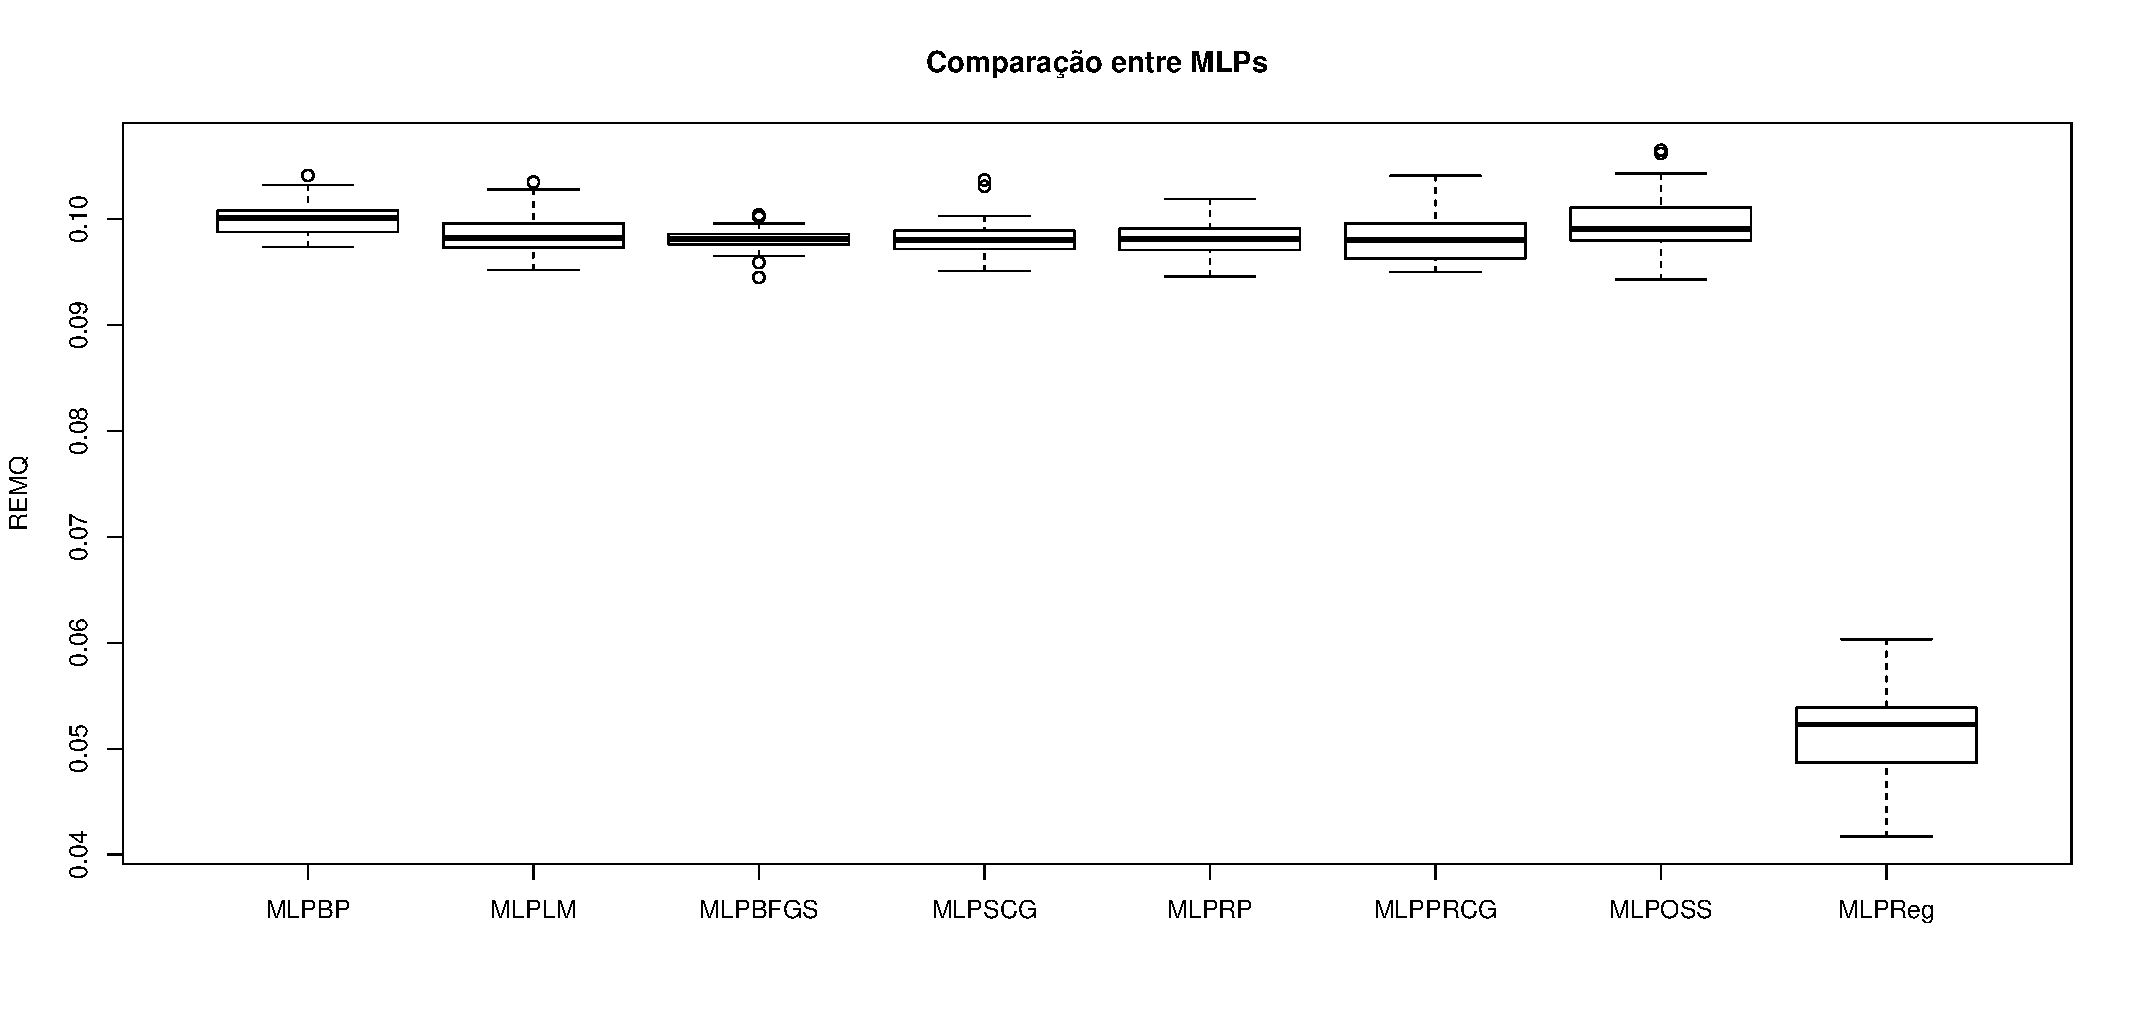
\includegraphics[trim = 1mm 10mm 1mm 1mm,clip,width=\columnwidth]{image/mlps_ex3.pdf}
  \caption{\textit{Boxplots} para erros normalizados de várias MLPs.}
  \label{fig:mlps_result}
\end{figure}

Na Figura \ref{fig:mlps_result}, os \textit{boxplots} da REMQ normalizada, após as previsões para as oito MLPs, são apresentados. A partir dessas informações, pode-se afirmar que a MLP chamada ``MLPRegressor" é a rede neural mais eficiente porém não tão precisa, de acordo com o experimento.

\section{MLP, SVM, RBF e ANFIS}

Após determinar uma MLP eficiente no experimento anterior, o quarto experimento tem o objetivo de eleger qual a melhor técnica baseada em Redes Neurais Artificiais, dentre as implementadas, para a previsão do impacto de riscos a partir da base de dados PERIL.

A Tabela \ref{tab:anns_descriptive} mostra a estatística descritiva da REMQ normalizada para as RNAs estudadas. Os valores de média, desvio padrão, mínimo e máximo, calculados para um modelo \textit{Neuro-Fuzzy} ANFIS, uma SVM (chamada ``SMORegressor"), uma rede RBF (chamada ``RBFRegressor") e para uma MLP (``MLPRegressor") mostram que o último algoritmo apresenta valores bem inferiores de média (0.0516), mínimo (0.0427) e máximo (0.0603). No entanto, o desvio padrão do ANFIS é menor (0.00003). Portanto, ``MLPRegressor" provou ser um método mais eficiente 52\% na média comparado ao ANFIS porém menos preciso, em comparação com as outras técnicas, para a estimativa do impacto de risco baseada na PERIL.

\begin{table}[b]
\caption{Estatísticas descritivas para erros normalizados de RNAs.}\label{tab:anns_descriptive} \centering
\begin{tabular}{|c|c|c|c|c|}
  \hline
   & ANFIS & SMOReg & RBFReg & MLPReg  \\
  \hline
  Média & 0,1079 & 0,09430 & 0,09004 & \textbf{0,0516}   \\
  \hline
  Desv. Padrão & \textbf{0,00003} & 0,00488 & 0,00432 & 0,0042   \\
  \hline
  Mínimo & 0,1078 & 0,08347 & 0,08024	 & \textbf{0,0427}   \\
  \hline
  Máximo & 0,1080 & 0,10284 & 0,09790 & \textbf{0,0603}   \\
  \hline
\end{tabular}
\end{table}

\begin{figure}[!b]
  \vspace{-0.2cm}
  \centering
  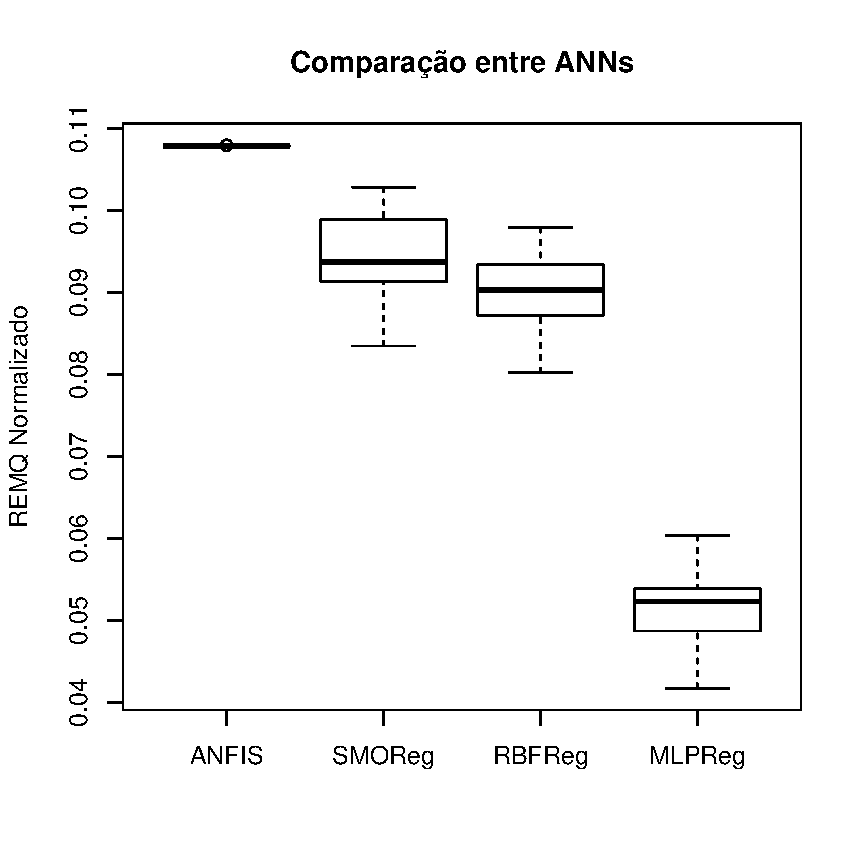
\includegraphics[trim = 1mm 12mm 1mm 1mm,clip,width=0.7\columnwidth]{image/anns_ex4.pdf}
  \caption{\textit{Boxplots} para os erros normalizados das RNAs.}
  \label{fig:anns_result}
\end{figure}

Na Figura \ref{fig:anns_result}, os \textit{boxplots} da REMQ normalizada, após as estimativas de impacto das RNAs, são apresentados. A partir dessas informações, pode-se afirmar que o ``MLPRegressor" é a RNA mais eficiente, porém ainda um pouco imprecisa, de acordo com essa comparação.

\begin{figure}[!h]
  \centering
  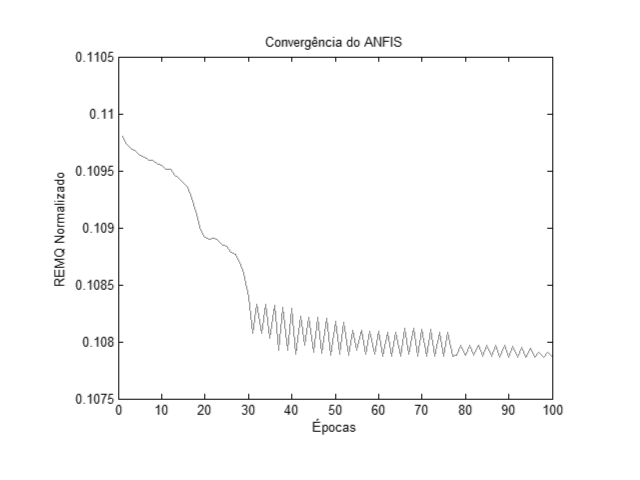
\includegraphics[trim = 1mm 12mm 1mm 8mm,clip,width=\columnwidth]{image/epocas.png}
  \caption{Gráfico de convergência do ANFIS.}
  \label{fig:anns_result_2}
\end{figure}

Na Figura \ref{fig:anns_result_2}, é apresentada a convergência do ANFIS, em termos da REMQ normalizada, para cada época durante o treinamento até ser interrompido, de acordo com a validação cruzada. Observa-se que o algoritmo encontrou um mínimo local e nele permaneceu preso até que o treinamento fosse interrompido. Logo, conclui-se que o ANFIS apresenta algumas limitações de convergência para essa base de dados.

\begin{figure}[!h]
  \vspace{-0.2cm}
  \centering
  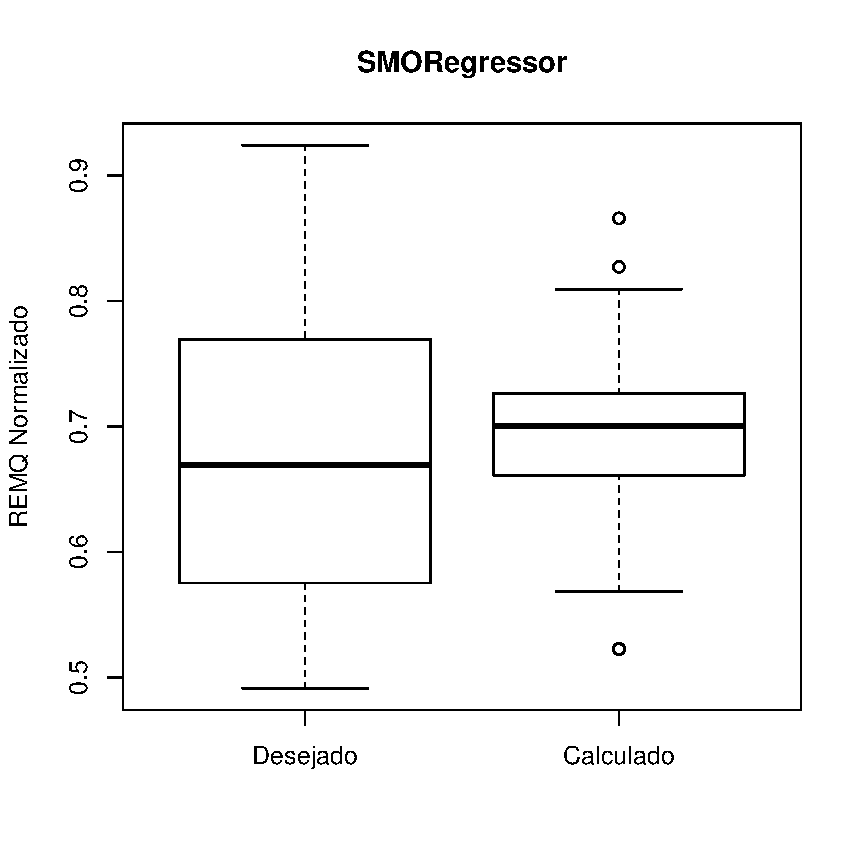
\includegraphics[trim = 1mm 12mm 1mm 1mm,clip,width=0.7\columnwidth]{image/smoreg_ex4.pdf}
  \caption{\textit{Boxplots} para previsões de impacto esperados e calculados para SVM.}
  \label{fig:anns_result_5}
\end{figure}

Na Figura \ref{fig:anns_result_5}, os \textit{boxplots} dos impactos esperados e calculados pelo algoritmo ``SMORegressor" de cinquenta amostras são apresentados. O resultado ideal é que os \textit{boxplots} das duas amostras fossem o mais semelhantes possível, respeitando a mediana, o intervalo inter-quartil e os valores de mínimo e máximo. A partir da informação apresentada, pode-se concluir que o \textit{boxplot} oriundo dos impactos calculados tentou representar mas distorceu em todas as medidas os impactos esperados.

\begin{figure}[!h]
  \vspace{-0.2cm}
  \centering
  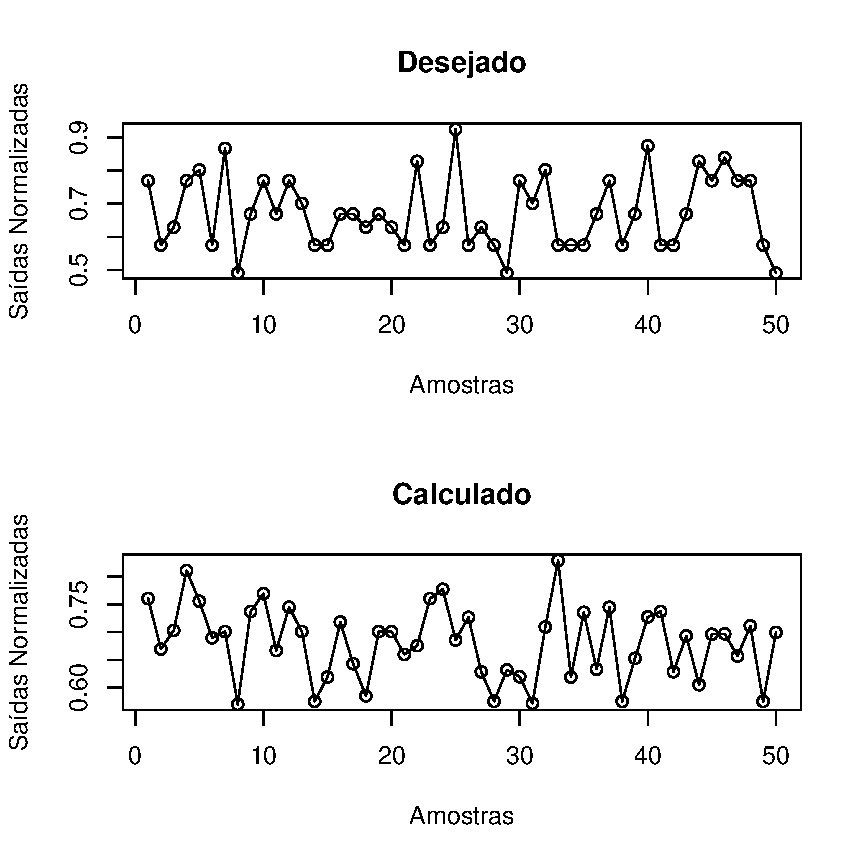
\includegraphics[width=0.7\columnwidth]{image/smoreg_ex4_2.pdf}
  \caption{Amostras de previsões de impacto esperado e calculado para SVM.}
  \label{fig:anns_result_6}
\end{figure}

Na Figura \ref{fig:anns_result_6}, as cinquenta primeiras amostras do subconjunto de testes e da saídas calculadas são apresentadas, graficamente. A partir desses gráficos, pode-se observar que o algoritmo ``SMORegressor" teve dificuldade em estimar os resultados esperados, quase não apresentando relação com eles.

\begin{figure}[!h]
  \vspace{-0.2cm}
  \centering
  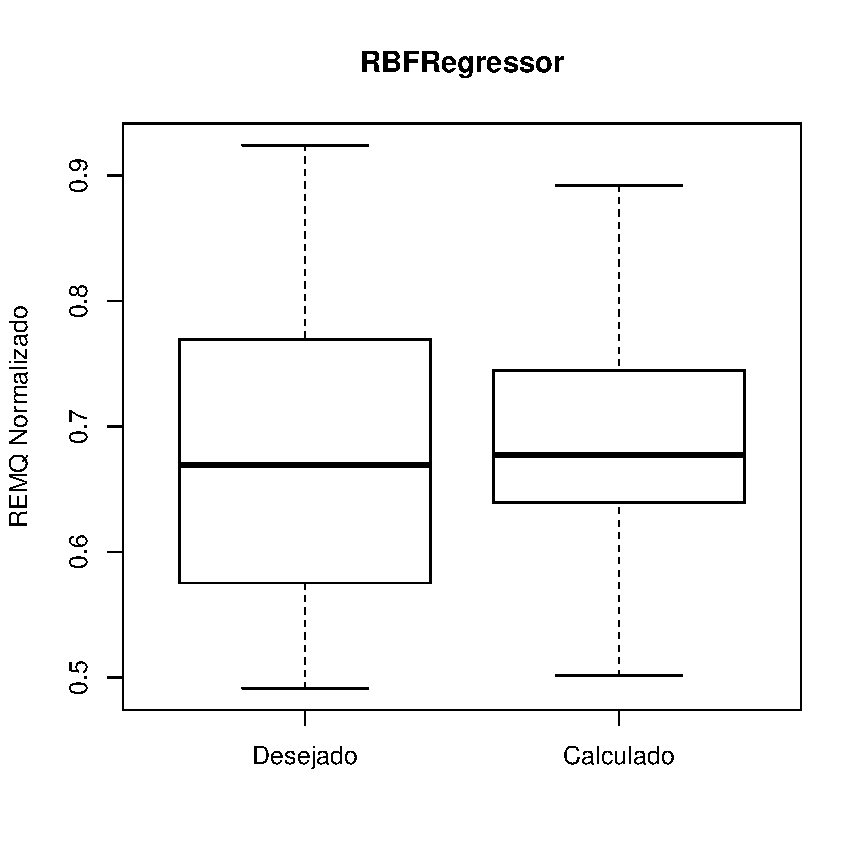
\includegraphics[trim = 1mm 12mm 1mm 1mm,clip,width=0.7\columnwidth]{image/rbfreg_ex4.pdf}
  \caption{\textit{Boxplots} para previsões de impactos desejados e calculados para RBF.}
  \label{fig:anns_result_3}
\end{figure}

Na Figura \ref{fig:anns_result_3}, os \textit{boxplots} dos impactos esperados e calculados pelo algoritmo ``RBFRegressor" de cinquenta amostras são apresentados. O resultado ideal é que os \textit{boxplots} das duas amostras fossem o mais semelhantes possível, respeitando a mediana, o intervalo inter-quartil e os valores de mínimo e máximo. A partir da informação apresentada, pode-se concluir que o \textit{boxplot} oriundo dos impactos calculados tentou representar mas distorceu no quartil inferior e nos valores máximos os impactos esperados.

\begin{figure}[!h]
  \vspace{-0.2cm}
  \centering
  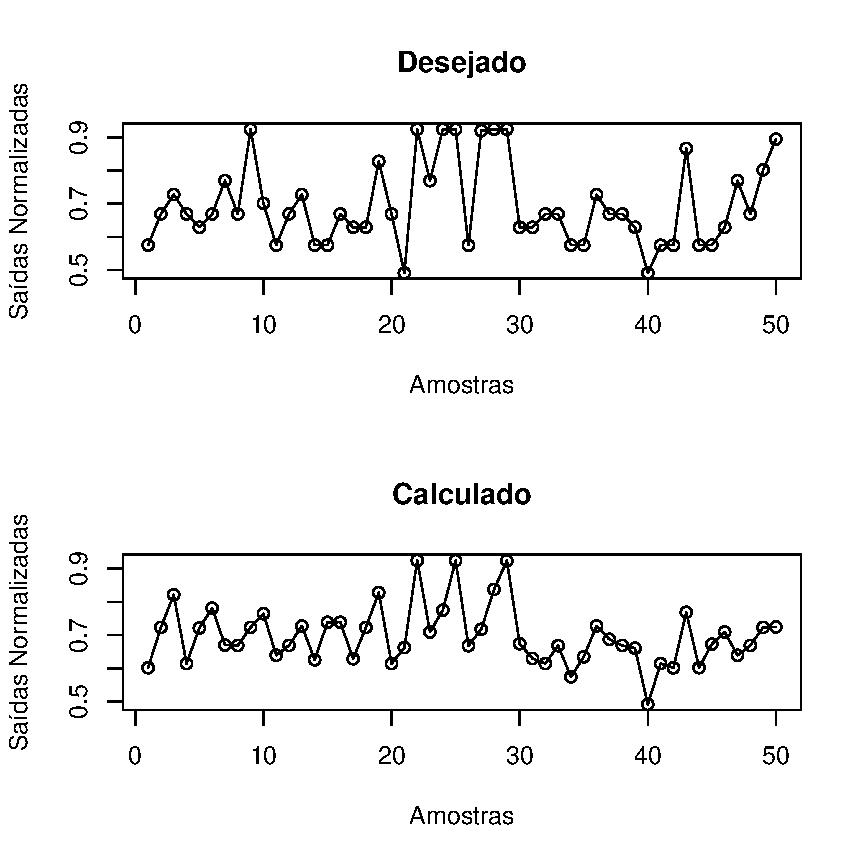
\includegraphics[width=0.7\columnwidth]{image/rbfreg_ex4_2.pdf}
  \caption{Amostras de previsões de impactos desejados e calculados para RBF.}
  \label{fig:anns_result_4}
\end{figure}

Na Figura \ref{fig:anns_result_4}, as cinquenta primeiras amostras do subconjunto de testes e das saídas calculadas são apresentadas, graficamente. A partir desses gráficos, pode-se observar que o algoritmo ``RBFRegressor" teve dificuldade em estimar os resultados esperados, principalmente os valores máximos e mínimos.

\begin{figure}[!h]
  \vspace{-0.2cm}
  \centering
  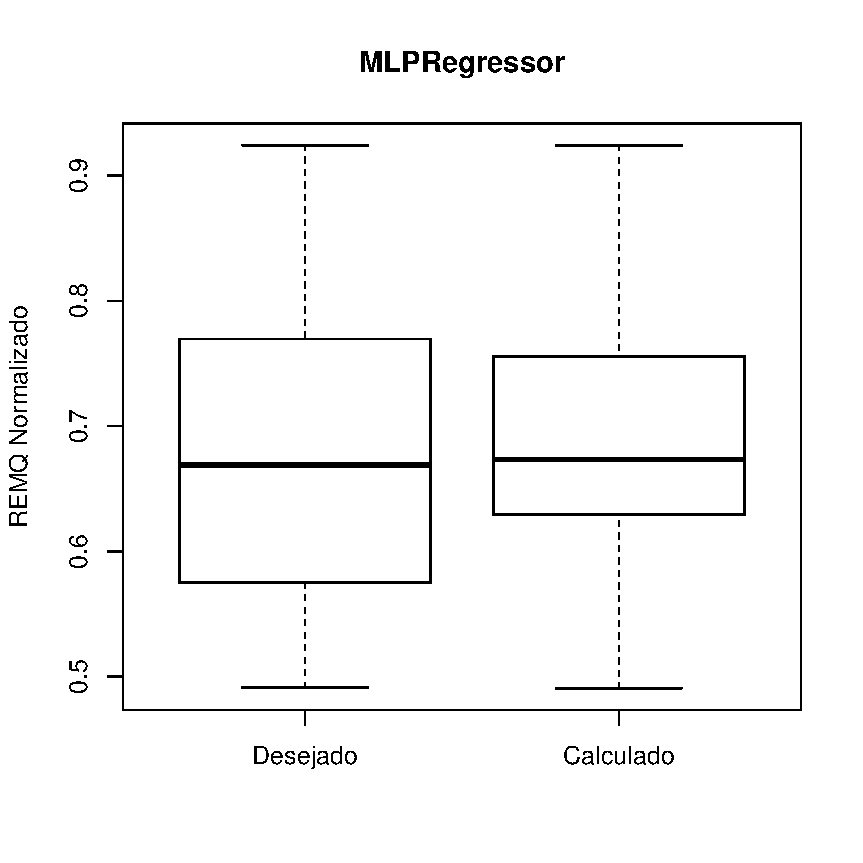
\includegraphics[trim = 1mm 12mm 1mm 1mm,clip,width=0.7\columnwidth]{image/mlpreg_ex4.pdf}
  \caption{\textit{Boxplots} para previsões de impacto esperados e calculados para MLPRegressor.}
  \label{fig:anns_result_7}
\end{figure}

Na Figura \ref{fig:anns_result_7}, os \textit{boxplots} dos impactos esperados e calculados pelo algoritmo ``MLPRegressor" de cinquenta amostras são apresentados. O resultado ideal é que os \textit{boxplots} das duas amostras fossem o mais semelhantes possível, respeitando a mediana, o intervalo inter-quartil e os valores de mínimo e máximo. A partir da informação apresentada, pode-se concluir que o \textit{boxplot} oriundo dos impactos calculados representou, porém com distorções principalmente no quartil inferior, os impactos esperados.

\begin{figure}[!h]
  \vspace{-0.2cm}
  \centering
  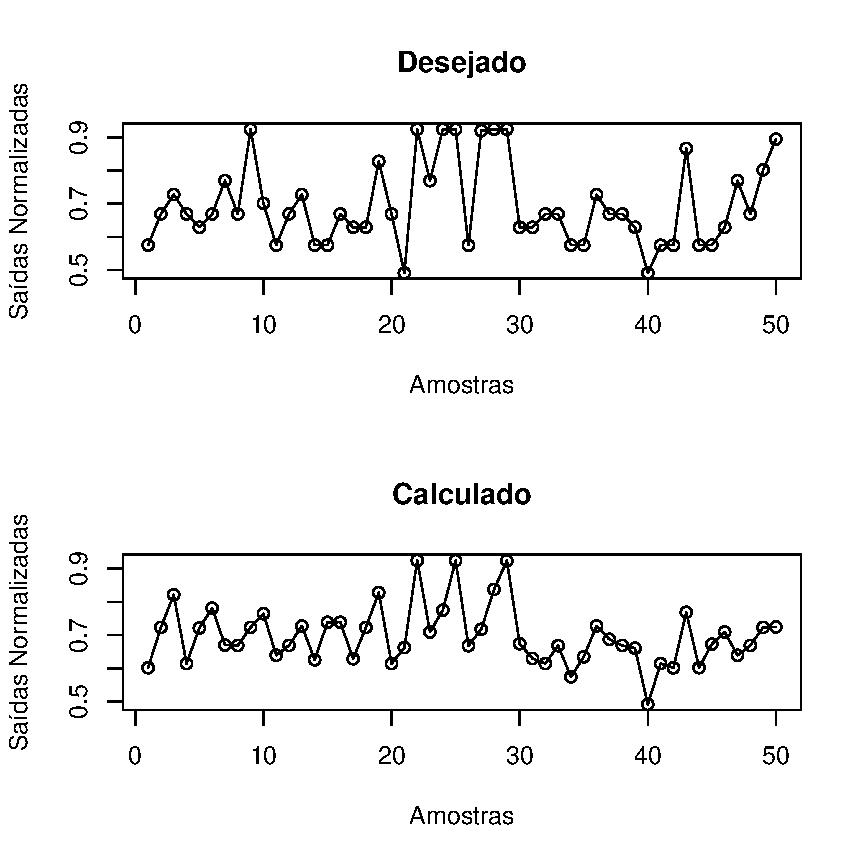
\includegraphics[width=0.7\columnwidth]{image/mlpreg_ex4_2.pdf}
  \caption{Amostras de previsões de impacto esperado e calculado para MLPRegressor.}
  \label{fig:anns_result_8}
\end{figure}

Na Figura \ref{fig:anns_result_8}, as cinquenta primeiras amostras do subconjunto de testes e das saídas calculadas são apresentadas, graficamente. A partir desses gráficos, pode-se observar que o algoritmo ``MLPRegressor" teve dificuldade em estimar os resultados esperados, porém tendeu a acompanhar os resultados.

\section{Validação do Melhor Modelo}

A Tabela \ref{tab:validacao_descriptive} mostra a estatística descritiva da REMQ normalizada para as RNAs estudadas. Os valores de média, desvio padrão, mínimo e máximo, calculados para um MRLM, uma Simulação de Monte Carlo(SMC), uma Análise PERT(PERT) e para uma MLP ``MLPRegressor"(MLPReg) mostram que o último algoritmo apresenta valores inferiores de média, desvio padrão, mínimo e máximo. Portanto, ``MLPRegressor" provou ser um método mais eficiente e relativamente preciso, em comparação com as outras técnicas, para a estimativa do impacto de risco baseada na PERIL.

\begin{table}[h]
\caption{Estatísticas descritivas para validação dos modelos selecionados.}\label{tab:validacao_descriptive} \centering
\begin{tabular}{|c|c|c|c|c|}
  \hline
   & MLR & MCS & PERT & MLPReg  \\
  \hline
  Méd & 0,09912 & 0,12640 & 0,07466 & \textbf{0,05168}   \\
  \hline
  DvP & 0,00794 & 0,01250 & 0,01438 & \textbf{0,00427}   \\
  \hline
  Mín & 0,08956 & 0,10410 & 0,04788	 & \textbf{0,04172}   \\
  \hline
  Máx & 0,10746 & 0,14950 & 0,09122 & \textbf{0,06035}   \\
  \hline
\end{tabular}
\end{table}

\begin{figure}[!h]
  \vspace{-0.2cm}
  \centering
  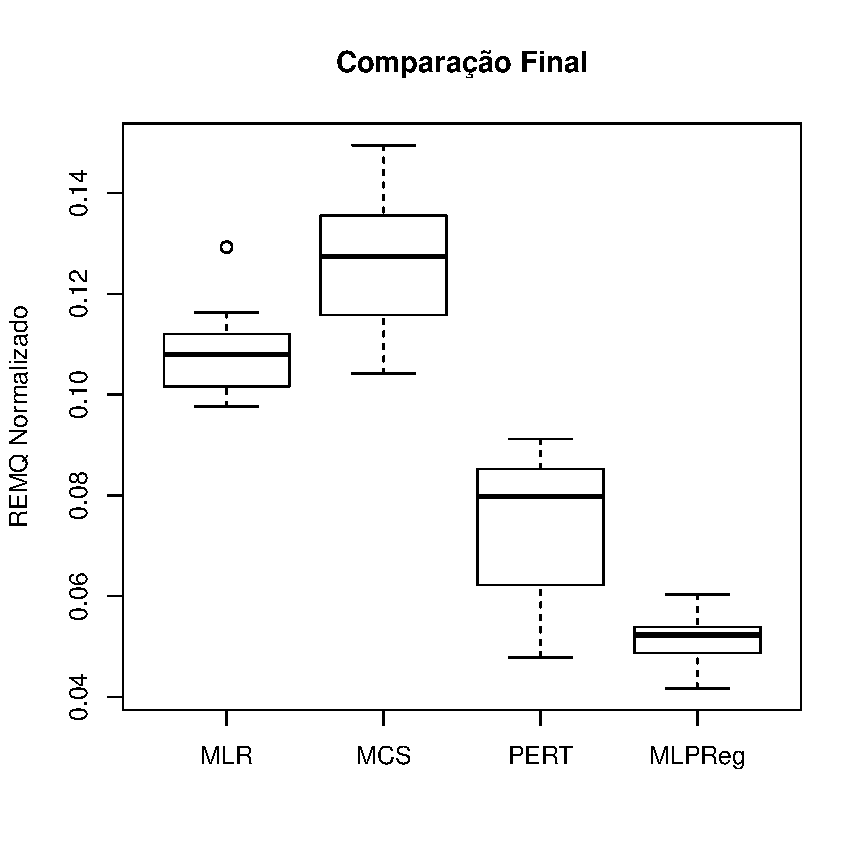
\includegraphics[trim = 1mm 12mm 1mm 1mm,clip,width=0.7\columnwidth]{image/validacao_ex5.pdf}
  \caption{\textit{Boxplots} dos erros normalizados para as técnicas de validação.}
  \label{fig:validacao_result}
\end{figure}

Na Figura \ref{fig:validacao_result}, os \textit{boxplots} da REMQ normalizado após as estimativas de impacto das RNAs são apresentados. A Simulação Monte Carlo(SMC) é imediatamente descartada da análise por apresentar erros maiores que o Modelo de Regressão Linear Múltipla (MLR); a Análise PERT (PERT) apresenta-se como uma abordagem simples e rápida para a estimativa do impacto de riscos, porém como é uma técnica estatística está sujeita a algumas situações que geram maiores erros na estimativa; já, o ``MLPRegressor" (MLPReg) apresenta os menores valores de média, desvio padrão, mínimo e máximo de erro. A partir dessas informações, pode-se afirmar que o ``MLPRegressor" é uma Rede Neural Artificial mais eficaz e precisa, comparada com o desempenho das outras RNAs.

A Tabela \ref{tab:teste_hipotese} apresenta os resultados dos Testes de Wilcoxon não-pareados para as RNAs estudadas. O símbolo $\Delta$ significa que a técnica à esquerda apresenta melhores resultados que a acima; diferentemente, o símbolo $\nabla$ significa que a técnica acima apresenta melhores resultados que à esquerda. Após analisar a tabela, pode-se afirmar que a ``MLPRegressor" foi melhor que a Análise PERT que, por sua vez, foi melhor que o Modelo de Regressão Linear Múltipla.

Não havia alguma expectativa para que o modelo ``MLPRegressor" fosse melhor que as outras técnicas.

%Teste de Hipótese
\begin{table}[h]
\caption{Testes de Hipótese para validação do melhor modelo.}\label{tab:teste_hipotese} \centering
\begin{tabular}{|c|c|c|c|c|}
  \hline
   & MLR & MCS & PERT & MLPReg  \\
  \hline
  MLR & - & $\Delta$ & $\nabla$ & $\nabla$   \\
  \hline
  MCS &  & - & $\nabla$ & $\nabla$   \\
  \hline
  PERT &  &  & - & $\nabla$   \\
  \hline
  MLPReg & & &  & -   \\
  \hline
\end{tabular}
\end{table}

\section{Previsão do Impacto e Intervalo de Confiança}

O último experimento consistiu na aplicação prática da metodologia proposta nesse estudo, com base no PERIL. Como alguns passos descritos na metodologia foram seguidos nos experimentos anteriores, resta somente a geração de um intervalo de confiança que é a informação compreendida pelos gerentes de projetos, analistas de projetos e de riscos.

A aplicação do intervalo de confiança irá determinar a qualidade dos resultados gerados. A partir dos resultados apresentados pelo modelo, foi gerado um intervalo que, para uma determinada previsão, teve 95 \% de chances de conter o valor real. Para isso, será utilizado o método de máxima verossimilhança.

O método de máxima verossimilhança considera que existem duas fontes de incertezas para um modelo de previsão. O primeiro, o $\sigma_v$, é a variância do ruído, e o segundo, $\sigma_w$, é a variância da incerteza. O $\sigma_v$ representa a variância dos erros gerados pelo conjunto de validação cruzada na fase de treinamento. Esses valores seguem uma distribuição normal e possuem média zero. Já o $\sigma_w$ é referente à variância de incerteza do modelo e é calculada a partir da utilização do modelo para prever os erros gerados pela própria rede.

Assume-se que essas duas fontes de erro são independentes. Então o cálculo da variância total do modelo é dado pela Equação \ref{eq:var_intervalo}.

\begin{equation}
\label{eq:var_intervalo}
\sigma^{2}_{total} = \sigma^{2}_{v} + \sigma^{2}_{w}.
\end{equation}

No processo de validação cruzada do modelo, calcula-se o $\sigma_v$ que é a variância dos erros. Para cada entrada do conjunto calcula-se o erro e ao final do processo a média desses erros e extrai-se sua variância usando a Equação \ref{eq:var_validacao} \label{symbol:var_validacao}.

\begin{equation}
\label{eq:var_validacao}
\sigma_v = \frac{1}{n-1} \sum_{n}^{i=1} (Erro_i - \overline{Erro})^2 , 
\end{equation}
onde, $n$ é a quantidade de valores; $Erro_i$ é o erro referente à entrada i; $\overline{Erro}$ é a média dos erros.

Para calcular o $\sigma_w$, armazenou-se os erros para todas as entradas utilizadas no treinamento da rede, incluindo dados de treinamento e validação cruzada. Com esses dados devidamente armazenados e normalizados, criou-se um novo modelo, com novos pesos e novas ligações. Esse modelo teve como objetivo, ou seja, valores desejados, os erros gerados pelo modelo anterior. O $\sigma_w$ será calculado utilizando a mesma fórmula utilizada para o $\sigma_v$. A diferença está na quantidade de dados, pois, para o $\sigma_w$ serão utilizados todos os erros de todos os conjuntos, não só o de validação cruzada.

Tendo o $\sigma_v$ e $\sigma_w$ calculados, pode-se calcular o $\sigma_total$. Este foi utilizado para calcular o intervalo de confiança a partir da Equação \ref{eq:intervalo_confianca}.

\begin{equation}
\label{eq:intervalo_confianca}
x - t * \sigma_total < x < x + t * \sigma_total , 
\end{equation}
onde, $x$ foi o valor calculado pela rede e $t$ foi o valor extraído da tabela de t de Student para o maior grau de liberdade possível para um intervalo de 95\% de chances de conter o valor real, como exibido na Tabela \ref{tab:lm_descriptive}.

\begin{table}[h]
\caption{Tabela T de Student}\label{tab:t-student} \centering
\begin{tabular}{|c|c|c|c|c|}
  \hline
  \multicolumn{5}{|c|}{$P(t_n \leq x)$}  \\
  \hline
  \textbf{n} & 0,750 & 0,900 & 0,950 & 0,975  \\
  \hline
  30 & 0,683 & 1,310 & 1,697 & 2,042   \\
  \hline
  40 & 0,681 & 1,303 & 1,684 & 2,021   \\
  \hline
  60 & 0,679 & 1,296 & 1,671 & 2,000   \\
  \hline
  120 & 0,677 & 1,289 & 1,658 & 1,980   \\
  \hline
  $\infty$ & 0,674 & 1,284 & 1,645 & \textbf{1,960}   \\
  \hline
\end{tabular}
\end{table}

\section{Considerações Finais}

Nesse trabalho, utiliza-se a validação cruzada por divisão de amostras balanceadas e gera-se aleatoriamente os valores de cada subconjuntos (treinamento, validação e testes). Já que utiliza-se um algoritmo de otimização (PSO), a avaliação do desempenho de cada partícula representa o processamento por completo do pré-processamento dos dados e a execução da estimativa do impacto do risco de cada modelo avaliado. 

Portanto, são geradas milhares de milhares de subconjuntos de dados a serem processados por cada modelo com diversas configurações de parâmetros, ajustados pelo PSO. Partindo desse ponto, decidiu-se não investigar outros métodos de validação cruzada como: o \textit{K-Fold cross-validation}, a distribuição por \textit{fold}, a distribuição do erro por posição geográfica e a divisão dos erros por posição geográfica nos \textit{folds}.

Além disso, os dados também foram ``binarizados" de modo que para cada classe, apenas uma classe de valor numérico tenha um dígito ``1" na entrada. Dessa forma, obtém-se 33 variáveis de entrada ``binarizadas" ao invés das 12 iniciais. Porém, durante as simulações tivemos um aumento considerável do consumo de recursos computacionais e tempo para obter resultados estatisticamente iguais. Ademais para o algoritmo ANFIS, que é implementado no Matlab, houve erro de processamento, e assim, não obteve-se resultados. 

\pagebreak
